\chapter{ND-GAr}
\label{chapter:nd_gar}

ND-GAr is a magnetised, high-pressure gaseous argon TPC (HPgTPC), surrounded by an electromagnetic calorimeter (ECal) and a muon detector (commonly refer to as $\mu$ID). A detailed discussion on the requirements, design, performance and physics of ND-GAr can be found in the DUNE ND CDR \cite{DUNE2021NDCDR} and the ND-GAr whitepaper (cite).

In DUNE Phase II ND-GAr will fulfill the role of TMS, measuring the momentum and sign of the charged particles exiting ND-LAr. Additionally, it will be able to measure neutrino interactions inside the HPgTPC, achieving lower energy thresholds than those of the ND and FD LArTPCs. By doing so ND-GAr will allow to constrain the relevant systematic uncertainties for the LBL analysis even further.

The goal of the present chapter is to review the requirements that the physics program of DUNE impose on ND-GAr, present the current status of its design and describe the GArSoft package, its simulation and reconstruction software.

\section{Requirements}

The primary requirement for ND-GAr is to the measure the momentum and charge of muons from $\nu_{\mu}$ and $\bar{\nu}_{\mu}$ CC interactions in ND-LAr, in order to measure their energy spectrum. To achieve the sensitivity to the neutrino oscillation parameters described in the DUNE FD TDR Volume II \cite{DUNE2020TDR2} ND-GAr should be able to constrain the muon energy within a $1\%$ uncertainty or better. The main constraint will come from the calibration of the magnetic field, performed using neutral kaon decays in the HPgTPC.

Another requirement for ND-GAr is the precise measurement of neutrino interactions on argon for the energies relevant to the neutrino oscillation program. The goal is to constrain the cross section systematic uncertainties in the regions of phase space that are not accessible to ND-LAr. This requires the kinematic acceptance for muons in ND-GAr to exceed that of ND-LAr, being comparable to the one observed in the FD.

ND-GAr should also be able to the relationship between true and reconstructed energy from neutrino interactions on argon with low thresholds, being sensitive to particles that are not observed or may be misidentified in ND-LAr. In particular, ND-GAr needs to have low tracking thresholds in order to measure the spectrum of pions and protons produced in final-state interactions (FSI). It also must be able to accurately measure the pion multiplicity in 1, 2 and 3 pions final states, to inform the pion mass correction in the LArTPCs.

\section{Reference design}

The final design of ND-GAr is still under preparation. However, a preliminary baseline design was in place at the time of the ND CDR. This section summarises the main features of that design, as it is also the one used for the default geometry in our simulation. A DUNE Phase II whitepaper, discussing the different options under consideration for the ND-GAr design, is in progress. 

\subsection{HPgTPC}

The reference design for the ND-GAr HPgTPC follow closely that of the ALICE TPC. It is a cylinder with a central high-voltage cathode, generating the electric field for the two drift volumes, with a maximum drift distance of $2.5~\mathrm{m}$ each. The anodes will be instrumented with charge readout chambers. The original design repurposed the multi-wire proportional readout chambers of ALICE, however the current R\&D efforts focus on a gas electron multiplier option instead. Fig. \ref{fig:alice_tpc} shows a schematic diagram of the ALICE TPC design. The basic ND-GAr geometry will resemble this, except for the inner field cage.

\begin{figure}[t]
	\centering
	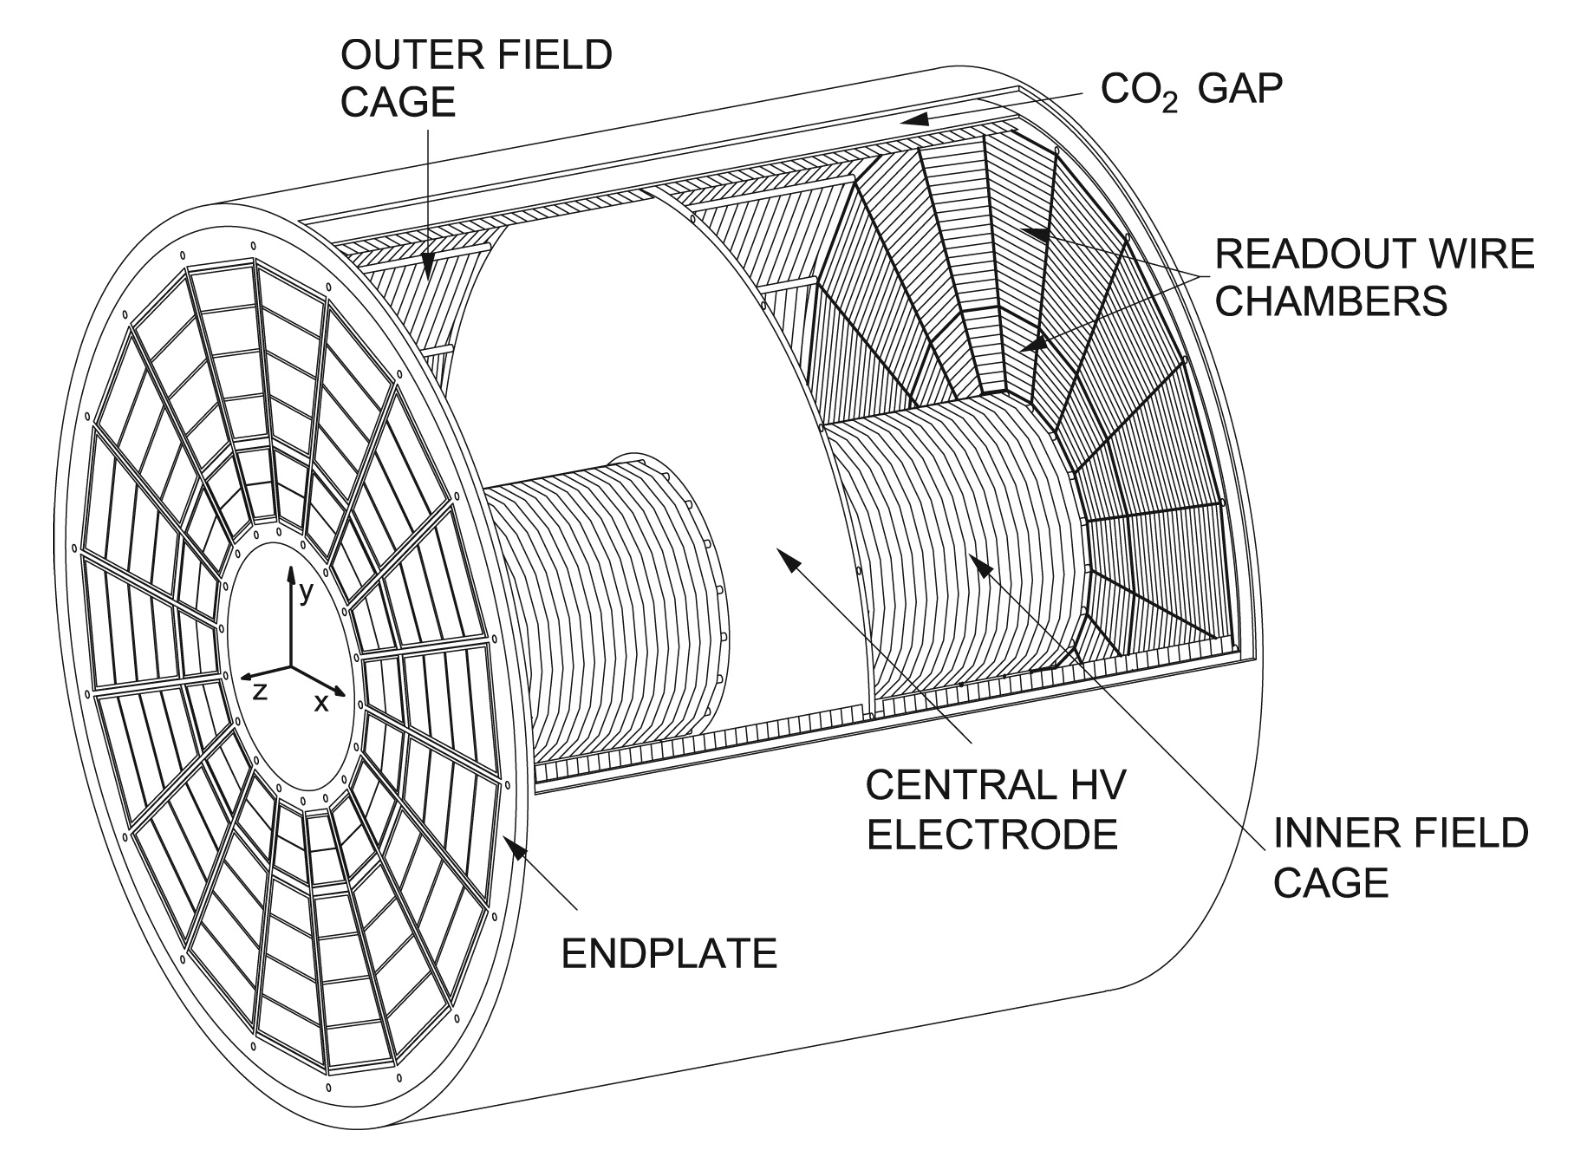
\includegraphics[width=0.7\linewidth]{Images/ND-GAr/alice_tpc}
	\caption[Diagram of the ALICE TPC, showing the two drift chambers, inner and outer field cages and readout chambers.]{Diagram of the ALICE TPC, showing the two drift chambers, inner and outer field cages and readout chambers. Figure taken from Ref. \cite{DUNE2020TDR1}.}
	\label{fig:alice_tpc}
\end{figure}

It will use a 90-10 molar fraction argon-CH$_{4}$ mixture at $10~\mathrm{bar}$. With this baseline gas mixture light collection is not possible, as the quenching gas absorbs most of the VUV photons. Additional R\&D efforts are underway, to understand if different mixtures allow for the light signal to be used to provide a $t_{0}$ while maintainig stable charge gain.

\subsection{ECal}

\begin{figure}[t]
	\centering
	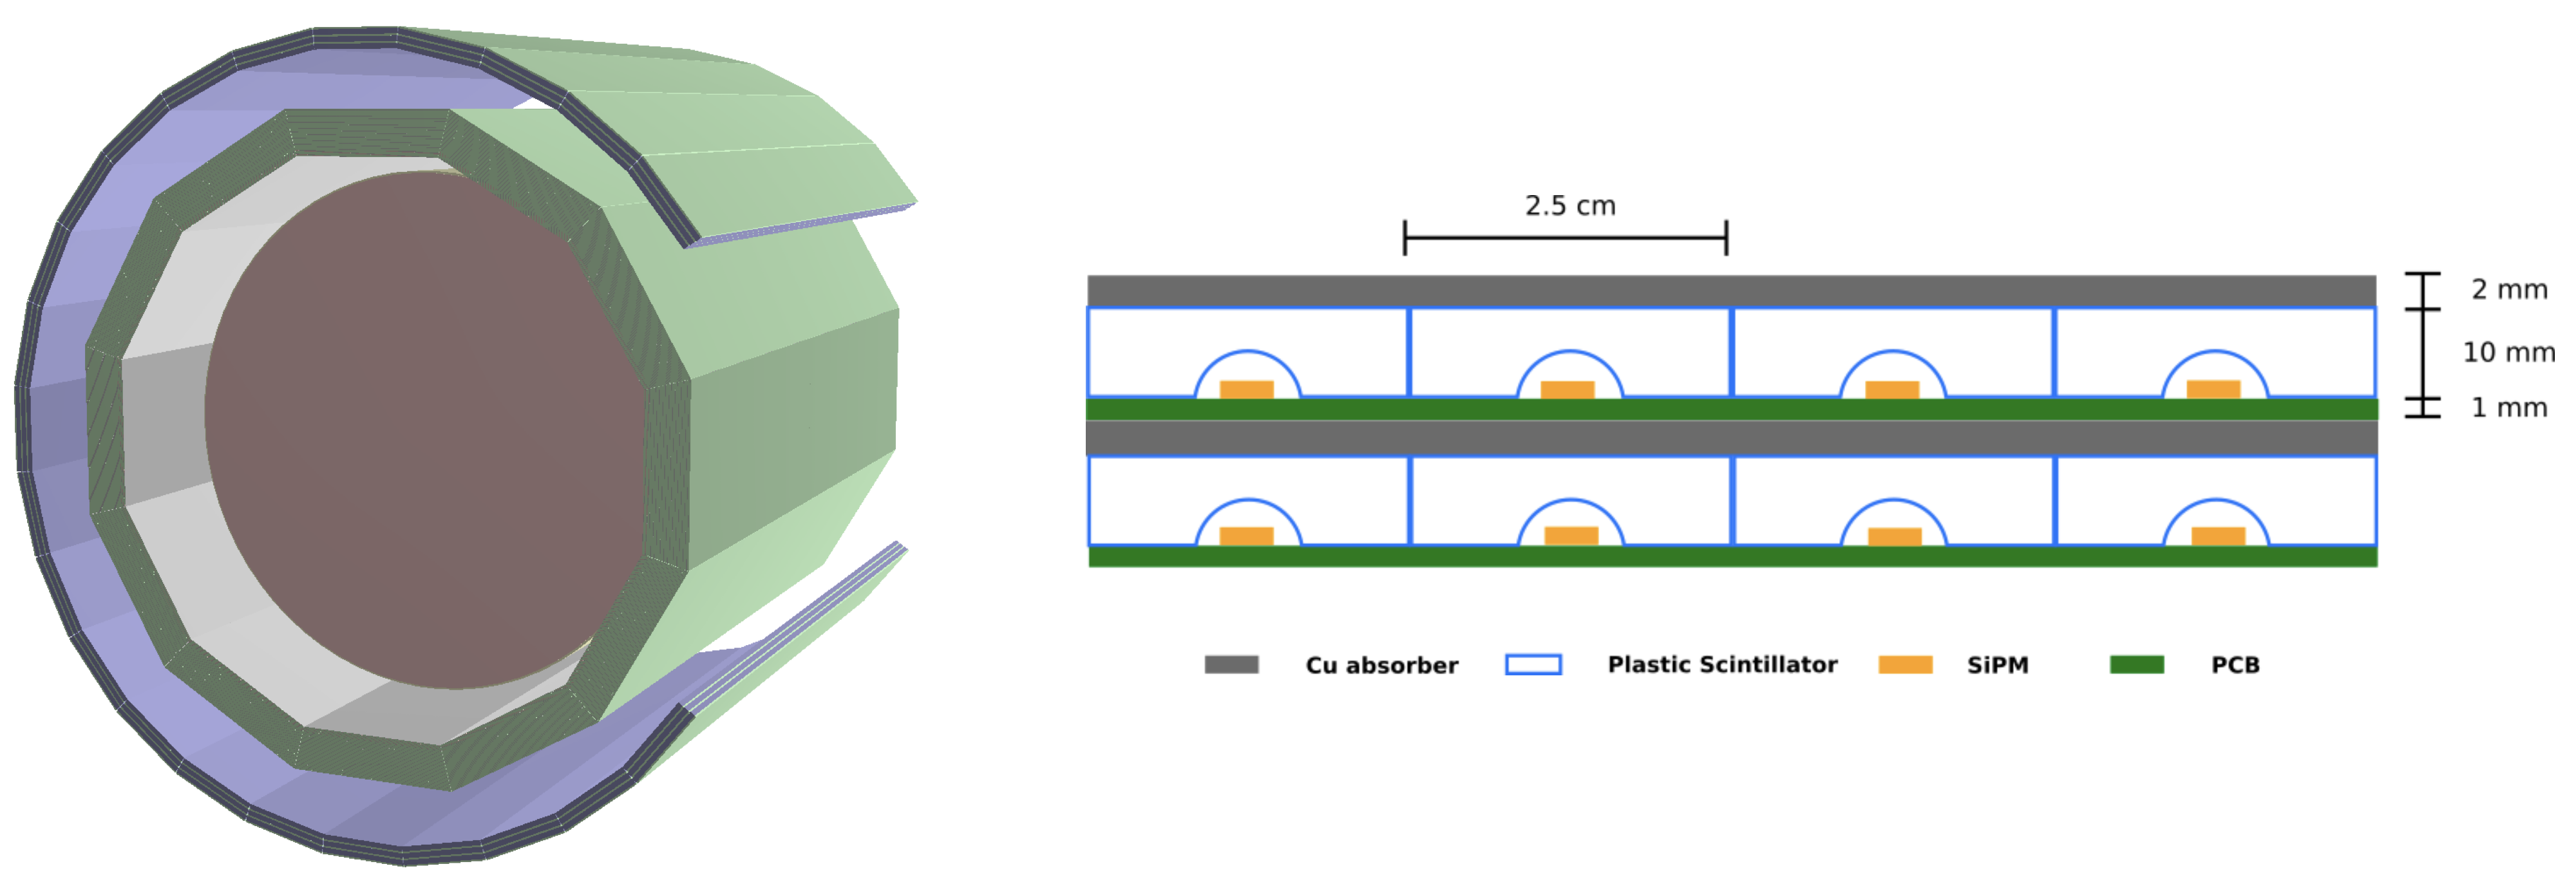
\includegraphics[width=0.99\linewidth]{Images/ND-GAr/ndgar_ecal}
	\caption[Diagram of the ALICE TPC, showing the two drift chambers, inner and outer field cages and readout chambers.]{View of the 12-sided ECal barrel and outer muon tagger geometries (left) and layout of the ECal tile layers for the $2~\mathrm{mm}$ Cu, $10~\mathrm{mm}$ scintillator option (right). Figure adapted from Ref. \cite{DUNE2020TDR1}.}
	\label{fig:ndgar_ecal}
\end{figure}

The main role of the ND-GAr ECal is the calorimetric measurement of the electron energies and the reconstruction of photons, in particular those from neutral pion decays. Also, the ECal is able to provide a $t_{0}$ timestamp for neutrino interactions, by associating its activity to the tracks in the HPgTPC. The ECal will also be able to perform neutron reconstruction using time of flight and reject external backgrounds, thanks to its sub-nanosecond time resolution.

The ECal design features three independent subdetectors, two end caps at each side and a barrel surrounding the HPgTPC. Each of the detectors is divided in modules, which combine alternating layers of plastic scintillator and absorber material readout by SiPMs. The inner scintillator layers consist of $2.5\times2.5~\mathrm{cm}^{2}$ high-granularity tiles, whereas the outer ones are made out of $4~\mathrm{cm}$ wide cross-strips spanning the whole module length. The current barrel geometry consists of 8 tile layers and 34 strip layers, while the end caps feature 6 and 36 respectively. The thickness of the scintillator layers is $7~\mathrm{mm}$ and $5~\mathrm{mm}$ for the Pb absorber layers. The 12-sided geometry of the ECal barrel (left) and the layout of the tile layers (left)\footnote{The figure shows the layout of the tile layers for a previous design with $2~\mathrm{mm}$ Cu absorber and $10~\mathrm{mm}$ plastic scintillator, as mentioned in the text the current choice is $5~\mathrm{mm}$ Pb absorber and $7~\mathrm{mm}$ scintillator.} can be seen in Fig. \ref{fig:ndgar_ecal}.

\subsection{Magnet}

The ND-GAr magnet design, know as the Solenoid with Partial Yoke (SPY), consists of two coupled solenoids with an iron return yoke. The idea behind the design is to have a solenoid as thin as possible, as well as a return yoke mass distribution that minimises the material budget between ND-LAr and ND-GAr. The magnet needs to provide a $0.5~\mathrm{T}$ field in the direction perpendicular to the beam, parallel to the drift electric field. It needs to host the pressure vessel and the surrounding ECal, which points to a inner diameter of $\sim6.4~\mathrm{m}$.

The solenoid is a single layer coil, based on niobium titanium superconducting Rutherford cable. The total length of the coil is $7.5~\mathrm{m}$. The bobbin will be split in four segments grouped in pairs with two identical cryostats, connected in series. The iron yoke features an aperture in the upstream side to allow the muons coming from ND-LAr. Still, its material will be enough to reduce the magnetic field reaching SAND, and also stop the charged pions produced inside the HPgTPC.

\subsection{Muon system}

The design of the ND-GAr muon system is still in a preliminary stage. Its role is to distinguish between muons and pions punching through the ECal. This is especially important for wrong-sign determination, to separate these from neutral current events.

In its current form, the muon system consists of three layers of longitudinal sampling structures. It alternates $10~\mathrm{cm}$ Fe absorber slabs with $2~\mathrm{cm}$ plastic scintillator strips. The transverse granularity required is still under study.

\section{GArSoft}

GArSoft is a software package developed for the simulation and reconstruction of events in ND-GAr. It is inspired by the LArSoft toolkit used for the simulation of LArTPC experiments, like the DUNE FD modules. It is based on \texttt{art}, the framework for event processing in particle physics experiments \cite{ART}. Other of its main dependencies are \texttt{ROOT}, \texttt{NuTools}, \texttt{GENIE} and \texttt{Geant4}. It allows the user to run all the steps of a generation-simulation-reconstruction workflow using FHiCL configuration files.

\subsection{Event generation}

The standard generator FHiCLs in GArSoft run the event generation and particle propagation simulation (i.e. Geant4) in the same job by default. However, it is possible to split them up if needed. The current version of GArSoft provides five different event generators, each of them producing \texttt{simb::MCTruth} products defined in \texttt{NuTools}. The available modules are:
\begin{itemize}
	\item \texttt{SingleGen}: particle gun generator. It produces the specified particles with a given distribution of momenta, initial positions and angles.
	\item \texttt{TextGen}: text file generator. The input file must follow the \texttt{hepevt} format\footnote{In brief, each event contains at least two  lines.  The first line contains two entries, the event number and the number of particles in the event. Each following line contains 15 entries to describe each particle. The entries are: status code, pdg code for the particle, entry of the first mother for this particle, entry of the second mother for this particle, entry of the first daughter for this particle, entry of the second daughter for this particle, x component of the particle momentum, y component of the particle momentum, z component of the particle momentum, energy of the particle, mass of the particle, x component of the particle initial position, y component of the particle initial position, z component of the particle initial position and time of the particle production.}, the module simply copies this to \texttt{simb::MCTruth} data products.
	\item \texttt{GENIEGen}: GENIE neutrino event generator. The module runs the neutrino-nucleus interaction generator using the options specified in the driver FHiCL file (flux file, flavour composition, number of interactions per event, $t_{0}$ distribution, ...). Current default version is \texttt{v3_04_00}.
	\item \texttt{RadioGen}: radiological generator. It produces a set list of particles to model radiological decays. Not tested.
	\item \texttt{CRYGen}: cosmic ray generator. The module runs the CRY event generator with a configuration specified in the FHiCL file (latitude and altitude of detector, energy threshold, ...). Not tested.
\end{itemize}

The module \texttt{GArG4} searches for all the generated \texttt{simb::MCTruth} data products, using them as inputs to the Geant4 simulation with the specified detector geometry. A constant $0.5~\mathrm{T}$ magnetic field along the drift coordinate is assumed. The main outputs of this step are \texttt{simb::MCParticle} objects for the generated Geant4 particles, \texttt{gar::EnergyDeposit} data products for the energy deposits in the HPgTPC and \texttt{gar::CaloDeposit} data products for the energy deposits in the ECal and muon system.

\subsection{Detector simulation}

The standard detector simulation step in GArSoft is all run with a single FHiCL, but the different modules can be run independently as well. First the \texttt{IonizationReadout} module simulates the charge readout of the HPgTPC, and later the \texttt{SiPMReadout} module runs twice, once for the ECal and then for the muon system, with different configurations.

The \texttt{IonizationAndScintillation} module collects all the \texttt{gar::EnergyDeposit} data products, to compute the equivalent number of ionization electrons for each energy deposit. The \texttt{ElectronDriftAlg} module simulates the electron diffusion numerically both in the longitudinal and transverse directions and applies an electron lifetime correction factor. The induced charge on the nearest and neighbouring readout pads is modeled using the provided pad response functions. The digitisation of the data is then simulated with the \texttt{TPCReadoutSimAlg} module. By default, the ADC sampling rate used is $50.505~\mathrm{MHz}$. The resulting raw waveforms for each channel are stored with zero-suppression, in order to save memory and CPU time. The algorithms keep blocks of ADC values above a certain threshold, plus some adjustable additional early and late tick counts. The results of these three steps are \texttt{gar::raw::RawDigit} data products.

For the ECal and the muon system the \texttt{SiPMReadout} module calls either the \texttt{ECALReadoutSimStandardAlg} or \texttt{MuIDReadoutSimStandardAlg} modules. These take all the \texttt{gar::CaloDeposit} data products in the corresponding detector and do the digitisation depending on whether the hit was in a tile or strip layer. They include single photon statistics, electronic noise, SiPM saturation and time smearing. The resulting objects are \texttt{gar::raw::CaloRawDigit} data products.

\subsection{Reconstruction}

The reconstruction in GArSoft is also run as a single job by default. It first runs the hit finding, clustering, track fitting and vertex identification in the HPgTPC, followed by the hit finding and clustering in the ECal and muon system. After those it produces the associations between the associations between the tracks and the ECal clusters.

Focusing first on the HPgTPC reconstruction, the \texttt{CompressedHitFinder} module takes the zero-suppressed ADCs from the \texttt{gar::raw::RawDigit} data products. The reconstructed hits largely correspond to the above threshold blocks, however the hit finder identifies waveforms with more than one maximum, diving them in multiple hits if they dip below a certain threshold. The data products produced are of the form \texttt{gar::rec::Hit}. These are the inputs to the clustering of hits in the \texttt{TPCHitCluster} module. Hits close in space and time are merged, and the resulting centroids are found. This module outputs \texttt{gar::rec::TPCClusters} objects and associations to the input hits.

The following step prior to the track fitting is pattern recognition. The module called \texttt{tpcvechitfinder2} uses the \texttt{gar::rec::TPCClusters} data products to find track segments, typically called vector hits. They are identified by performing linear 2D fits to the positions of the clusters in a $10~\mathrm{cm}$ radius, one fit for each coordinate pair. A 3D fit defines the line segment of the vector hit, using as independent variable the one whose sum of (absolute value) slopes in the 2D fits is the smallest. The clusters are merged to a given vector hit if they are less than $2~\mathrm{cm}$ away from the line segment. The outputs are \texttt{gar::rec::VecHit} data products, as well as associations to the clusters. The \texttt{tpcpatrec2} module takes the \texttt{gar::rec::VecHit} objects to form the track candidates. The vector hits are merged together if their direction matches, their centers are within $60~\mathrm{cm}$ and their direction vectors point roughly to their respective centers. Once the clusters of vector hits are formed they are used to make a first estimation of the track parameters, simply taking three clusters along the track. The module produces \texttt{gar::rec::Track} data products and associations between these tracks and the clusters and vector hits.

The track is fitted by means of a Kalman filter in the \texttt{tpctrackfit2} module, using the position along the drift direction as the independent variable. Two different fits are performed per track, a forward and a backwards fit, each starting from one of the track ends. The Kalman filter state vector $(y,z,R,\phi,\mathrm{tan}\lambda)$ is estimated at each point along the track using a Bayesian update. The track parameters reported in the forward and backwards fits are the ones computed at the opposite end where the fit started. The main outputs of the track fit are the \texttt{gar::rec::Track} objects. Additionally, the module stores the fitted 3D positions along the track in the \texttt{gar::rec::TrackTrajectory} data products and the total charge and step sizes for each point also get stored in the form of \texttt{gar::rec::TrackIonization} objects.

After the tracking step, the \texttt{vertexfinder1} module looks at the reconstructed \texttt{gar::rec::Track} products, creating vertex candidates with the track ends that are within $12~\mathrm{cm}$ of each other. The vertices are then fitted using linear extrapolations from the different track ends associated. The results are \texttt{gar::rec::Vertex} data products, and associations to the tracks and corresponding track ends.

For the ECal and muon tagger, the \texttt{SiPMHitFinder} module runs twice with different configurations, adapted to the particular capabilities of both. The module simply takes the \texttt{gar::raw::CaloRawDigit} products, applies a calibration factor to convert the ADC counts to $\mathrm{MeV}$ and for the strip layer hits it calculates the position along the strip using the times recorded of both SiPMs. This module produces \texttt{gar::rec::CaloHit} data products. Next, these objects are used as inputs to the \texttt{CaloClustering} module. It merges the hits based on a simple nearest neighbours (NN) algorithm. For the resulting clusters it also computes the total energy and position of the centroid. The results are stored as \texttt{gar::rec::Cluster} data products, with associations to the hits.

The last step in the reconstruction is associating the reconstructed tracks in the HPgTPC to the clusters formed in the ECal and muon system. The \texttt{TPCECALAssociation} module checks first the position of the track end points, considering only the points that are at least $215~\mathrm{cm}$ away from the cathode or have a radial distance to the center greater than $230~\mathrm{cm}$. The candidates are propagated up to the radial position, in the case of clusters in the barrel, or the drift coordinate position, for the end cap cluster, of the different clusters in the collection using the track parameters computed at the end point. The end point is associated to the cluster if certain proximity criteria are met. This module creates associations between the tracks, the end points and the clusters. The criteria for the associations are slightly different for the ECal and the muon tagger.